%!TEX root=report.tex
\subsection{OLS}

The first part of the OLS analysis will examine the EWH at two specific locations. The second part will then focus on the entire world. The main purpose of the OLS analysis is to estimate the velocity and acceleration of the mass changes.

\subsubsection{Selected locations}

The two selected locations are:
\begin{itemize}
\item Greenland ($63.5^\circ$ N, $49.5^\circ$ W)
\item South Pole ($74.5^\circ$ S, $87.5^\circ$ W)
\end{itemize}
\begin{figure}[H]
	\centering
	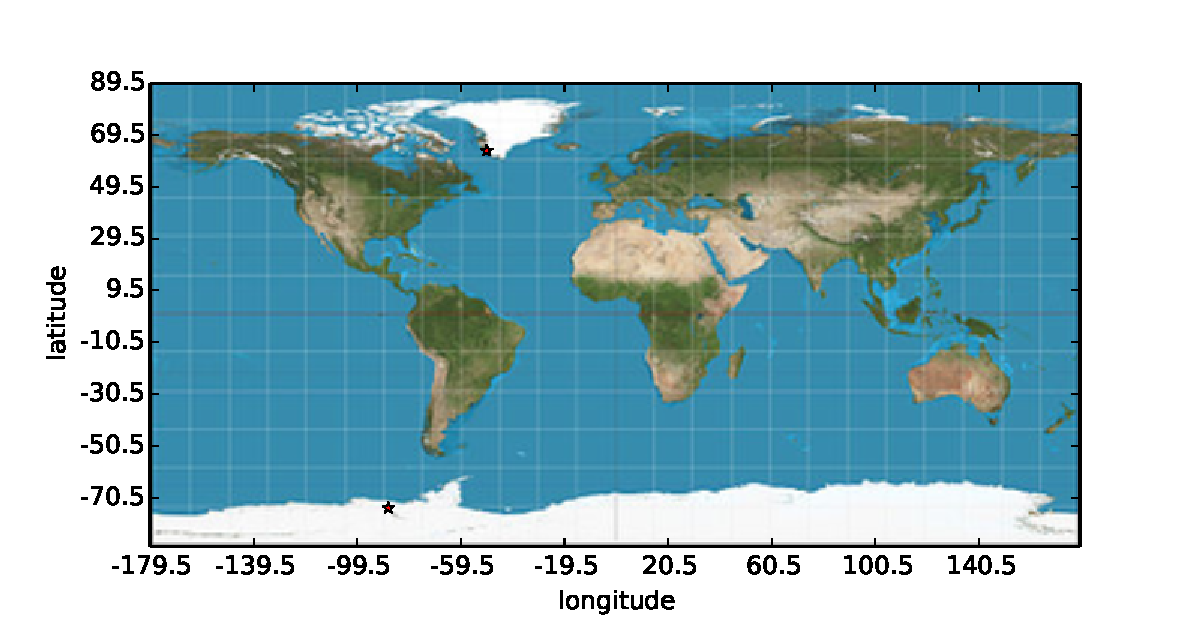
\includegraphics[height=6cm]{figures/ols-selected-map}
	\caption{The two selected locations, marked with a red star}
\end{figure}

\paragraph{Greenland}

At the west coast of Greenland a strong period trend can be observed, probably caused by the the ice melting over the summer and reappearing during the winter. This trend is seen in Figure \ref{fig:ols-selected-0-fit}. In order to estimate the velocity and acceleration of the EWH accurately, it is important that the periodic trend is caught by the $\sin(\cdot)$ and $\cos(\cdot)$ terms so that seasonal patterns do not interfere with the estimates.
\begin{figure}[H]
	\centering
	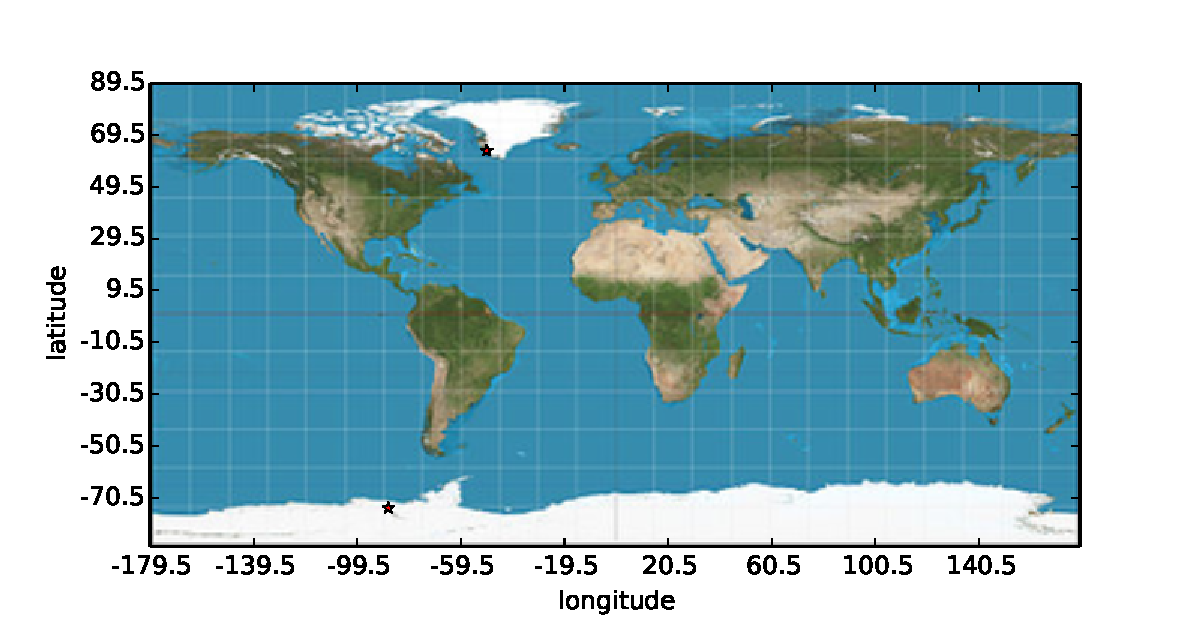
\includegraphics[width=\textwidth]{figures/ols-selected-0-fit}
	\caption{Measurements are blue, the OLS fit is red.}
	\label{fig:ols-selected-0-fit}
\end{figure}
 
From Figure \ref{fig:ols-selected-0-fit} it's seen that the period trend is caught by the model, however for some seasons (particular between 2008 and 2010) the fit is not very good. This is even more clear when looking at the residuals in Figure \ref{fig:ols-selected-0-residual}. From this it is clear that the residuals are far from white noise\todo{white noise vs normally distributed mean zero,constant variance and iid.}, which was one of the OLS assumptions.
\begin{figure}[H]
	\centering
	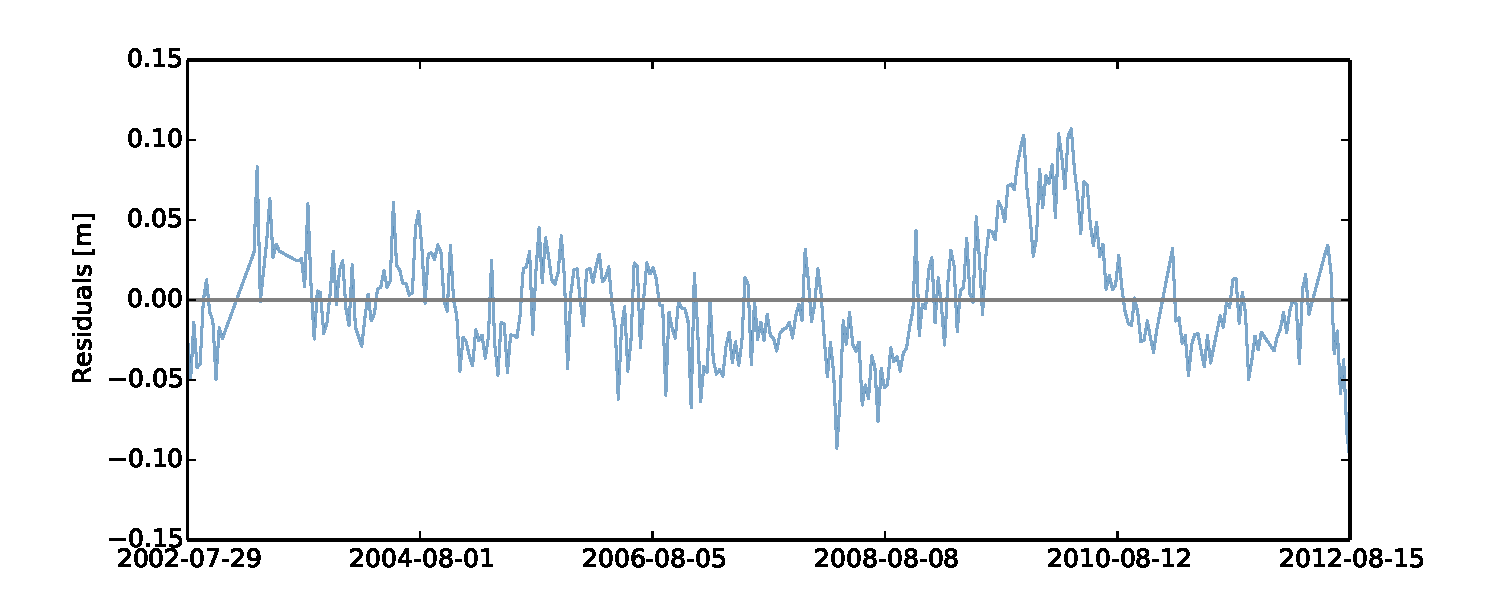
\includegraphics[width=\textwidth]{figures/ols-selected-0-residual}
	\caption{The OLS residuals are blue.}
	\label{fig:ols-selected-0-residual}
\end{figure}

In addition to the yearly season, when looking at the estimated OLS coefficients (Table \ref{table:ols-selected-0-paramters}) there also seems to be a half yearly season. Though strangely enough it is not very visible on the OLS fit (Figure \ref{fig:ols-selected-0-fit}). The remaining seasons are with 95\% confidence not significantly different from zero and for the purpose of getting a better estimate, it might be worth iteratively removing these parameters.
\begin{table}[H]
\centering
\centerline{\begin{tabular}{r|rr}
\hline
 name                                & estimate              & p-value   \\
\hline
 $intercept (1)$                     & $-1.77 \cdot e^{-01}$ & $0.000$   \\
 $vel. (t)$                          & $-2.24 \cdot e^{-04}$ & $0.000$   \\
 $acc. (0.5 \cdot t^2)$              & $-8.27 \cdot e^{-08}$ & $0.000$   \\
 $\cos(\sfrac{2\pi}{365.2} \cdot t)$ & $-1.35 \cdot e^{-02}$ & $0.000$   \\
 $\sin(\sfrac{2\pi}{365.2} \cdot t)$ & $-8.28 \cdot e^{-02}$ & $0.000$   \\
 $\cos(\sfrac{2\pi}{182.6} \cdot t)$ & $-5.86 \cdot e^{-03}$ & $0.045$   \\
 $\sin(\sfrac{2\pi}{182.6} \cdot t)$ & $-1.41 \cdot e^{-02}$ & $0.000$   \\
 $\cos(\sfrac{2\pi}{121.7} \cdot t)$ & $-5.01 \cdot e^{-03}$ & $0.089$   \\
 $\sin(\sfrac{2\pi}{121.7} \cdot t)$ & $-5.69 \cdot e^{-03}$ & $0.053$   \\
 $\cos(\sfrac{2\pi}{91.3} \cdot t)$  & $-5.49 \cdot e^{-03}$ & $0.060$   \\
 $\sin(\sfrac{2\pi}{91.3} \cdot t)$  & $-1.66 \cdot e^{-03}$ & $0.573$   \\
 $\cos(\sfrac{2\pi}{73.0} \cdot t)$  & $-2.19 \cdot e^{-03}$ & $0.455$   \\
 $\sin(\sfrac{2\pi}{73.0} \cdot t)$  & $-1.93 \cdot e^{-03}$ & $0.511$   \\
 $\cos(\sfrac{2\pi}{60.9} \cdot t)$  & $4.29 \cdot e^{-04}$  & $0.883$   \\
 $\sin(\sfrac{2\pi}{60.9} \cdot t)$  & $1.43 \cdot e^{-03}$  & $0.627$   \\
 $\cos(\sfrac{2\pi}{52.2} \cdot t)$  & $9.55 \cdot e^{-04}$  & $0.744$   \\
 $\sin(\sfrac{2\pi}{52.2} \cdot t)$  & $1.09 \cdot e^{-04}$  & $0.970$   \\
 $\cos(\sfrac{2\pi}{45.7} \cdot t)$  & $-3.08 \cdot e^{-04}$ & $0.916$   \\
 $\sin(\sfrac{2\pi}{45.7} \cdot t)$  & $-2.37 \cdot e^{-04}$ & $0.935$   \\
 $\cos(\sfrac{2\pi}{40.6} \cdot t)$  & $-2.02 \cdot e^{-03}$ & $0.491$   \\
\hline
\end{tabular}\hspace{1cm}\begin{tabular}{r|rr}
\hline
 name                               & estimate              & p-value   \\
\hline
 $\sin(\sfrac{2\pi}{40.6} \cdot t)$ & $8.48 \cdot e^{-04}$  & $0.772$   \\
 $\cos(\sfrac{2\pi}{36.5} \cdot t)$ & $1.54 \cdot e^{-03}$  & $0.599$   \\
 $\sin(\sfrac{2\pi}{36.5} \cdot t)$ & $-5.77 \cdot e^{-04}$ & $0.843$   \\
 $\cos(\sfrac{2\pi}{33.2} \cdot t)$ & $-5.95 \cdot e^{-04}$ & $0.839$   \\
 $\sin(\sfrac{2\pi}{33.2} \cdot t)$ & $-1.47 \cdot e^{-03}$ & $0.615$   \\
 $\cos(\sfrac{2\pi}{30.4} \cdot t)$ & $1.78 \cdot e^{-04}$  & $0.952$   \\
 $\sin(\sfrac{2\pi}{30.4} \cdot t)$ & $5.37 \cdot e^{-04}$  & $0.854$   \\
 $\cos(\sfrac{2\pi}{28.1} \cdot t)$ & $2.57 \cdot e^{-03}$  & $0.383$   \\
 $\sin(\sfrac{2\pi}{28.1} \cdot t)$ & $-6.35 \cdot e^{-04}$ & $0.827$   \\
 $\cos(\sfrac{2\pi}{26.1} \cdot t)$ & $3.16 \cdot e^{-04}$  & $0.914$   \\
 $\sin(\sfrac{2\pi}{26.1} \cdot t)$ & $-2.99 \cdot e^{-04}$ & $0.919$   \\
 $\cos(\sfrac{2\pi}{24.3} \cdot t)$ & $-7.23 \cdot e^{-04}$ & $0.804$   \\
 $\sin(\sfrac{2\pi}{24.3} \cdot t)$ & $3.33 \cdot e^{-04}$  & $0.910$   \\
 $\cos(\sfrac{2\pi}{22.8} \cdot t)$ & $-8.07 \cdot e^{-04}$ & $0.785$   \\
 $\sin(\sfrac{2\pi}{22.8} \cdot t)$ & $-6.93 \cdot e^{-04}$ & $0.811$   \\
 $\cos(\sfrac{2\pi}{21.5} \cdot t)$ & $-1.26 \cdot e^{-03}$ & $0.665$   \\
 $\sin(\sfrac{2\pi}{21.5} \cdot t)$ & $-7.28 \cdot e^{-04}$ & $0.803$   \\
 $\cos(\sfrac{2\pi}{20.3} \cdot t)$ & $-4.93 \cdot e^{-04}$ & $0.864$   \\
 $\sin(\sfrac{2\pi}{20.3} \cdot t)$ & $-9.94 \cdot e^{-06}$ & $0.997$   \\
                                    &                       &           \\
\hline
\end{tabular}}
\caption{Parameter estimates $\hat{\beta}$ and their p-values. }
\label{table:ols-selected-0-paramters}
\end{table}

\paragraph{South Pole}

Just like with Greenland there is a clear drop in mass as seen in Figure \ref{fig:ols-selected-1-fit}. Interestingly enough, there is no seasonal trend or at least it is not very strong. Also the existence of high frequency terms in the OLS regression, is more apparent. Though from the actual data it does not look like such periodic trends exist. This suggests that too many seasonal parameters have been used, thus causing some overfitting.
\begin{figure}[H]
	\centering
	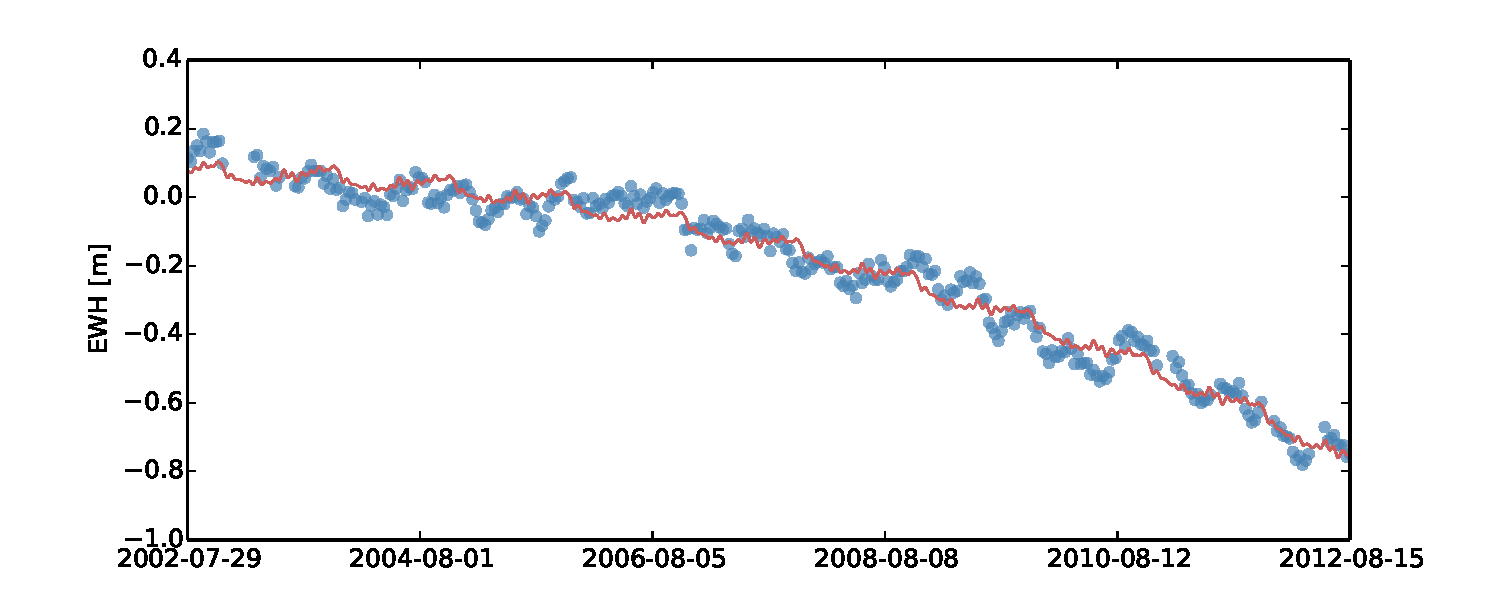
\includegraphics[width=\textwidth]{figures/ols-selected-1-fit}
	\caption{Measurements are blue, the OLS fit is red.}
	\label{fig:ols-selected-1-fit}
\end{figure}

When looking at the residuals in Figure \ref{fig:ols-selected-1-residual}, it is again clear that the residuals are far from being white noise\todo{white noise vs normally distributed, mean zero, constant variance and iid.}. There also seems to be some periodic trend in the residuals, although the beginnings and the endings of these seasons are quite hard to make out. 

\begin{figure}[H]
	\centering
	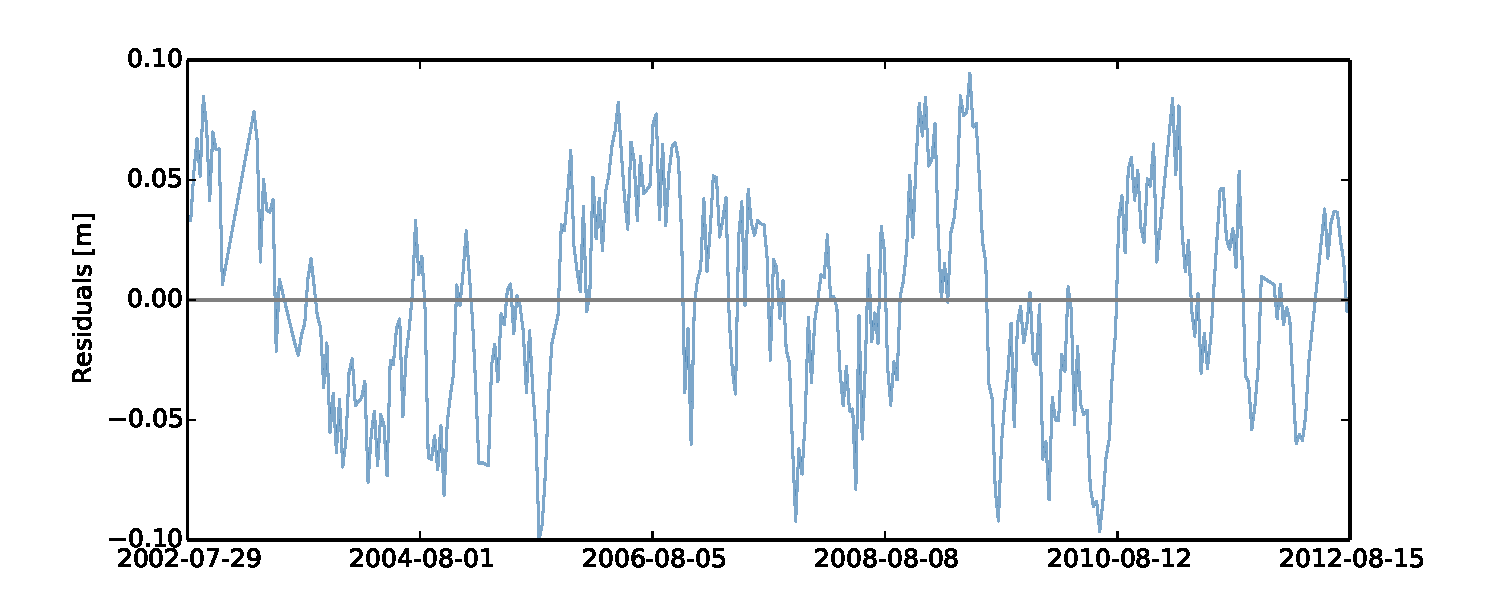
\includegraphics[width=\textwidth]{figures/ols-selected-1-residual}
	\caption{The OLS residuals are blue.}
	\label{fig:ols-selected-1-residual}
\end{figure}

Just as with Greenland many of the OLS terms are with 95\% confidence not significantly different from zero. Interestingly enough there is a yearly season when looking at Table \ref{table:ols-selected-1-paramters}, though it's very hard to make out from the OLS fit in Figure \ref{fig:ols-selected-1-fit}.

\begin{table}[H]
\centering
\centerline{\begin{tabular}{r|rr}
\hline
 name                           & estimate               & p-value   \\
\hline
 $intercept (1)$                & $-1.38 \cdot 10^{-01}$ & $0.000$   \\
 $vel. (t)$                     & $-2.26 \cdot 10^{-04}$ & $0.000$   \\
 $acc. (0.5 \cdot t^2)$         & $-1.24 \cdot 10^{-07}$ & $0.000$   \\
 $\cos(1 \cdot \omega \cdot t)$ & $1.69 \cdot 10^{-02}$  & $0.000$   \\
 $\sin(1 \cdot \omega \cdot t)$ & $1.42 \cdot 10^{-02}$  & $0.000$   \\
 $\cos(2 \cdot \omega \cdot t)$ & $-7.19 \cdot 10^{-03}$ & $0.046$   \\
 $\sin(2 \cdot \omega \cdot t)$ & $2.82 \cdot 10^{-03}$  & $0.440$   \\
 $\cos(3 \cdot \omega \cdot t)$ & $-4.36 \cdot 10^{-03}$ & $0.227$   \\
 $\sin(3 \cdot \omega \cdot t)$ & $-1.23 \cdot 10^{-03}$ & $0.732$   \\
 $\cos(4 \cdot \omega \cdot t)$ & $1.78 \cdot 10^{-03}$  & $0.619$   \\
 $\sin(4 \cdot \omega \cdot t)$ & $2.81 \cdot 10^{-03}$  & $0.437$   \\
 $\cos(5 \cdot \omega \cdot t)$ & $2.45 \cdot 10^{-03}$  & $0.496$   \\
 $\sin(5 \cdot \omega \cdot t)$ & $2.53 \cdot 10^{-03}$  & $0.484$   \\
 $\cos(6 \cdot \omega \cdot t)$ & $-1.60 \cdot 10^{-03}$ & $0.654$   \\
 $\sin(6 \cdot \omega \cdot t)$ & $-8.66 \cdot 10^{-04}$ & $0.811$   \\
 $\cos(7 \cdot \omega \cdot t)$ & $8.95 \cdot 10^{-04}$  & $0.803$   \\
 $\sin(7 \cdot \omega \cdot t)$ & $-3.27 \cdot 10^{-03}$ & $0.364$   \\
 $\cos(8 \cdot \omega \cdot t)$ & $1.62 \cdot 10^{-03}$  & $0.652$   \\
 $\sin(8 \cdot \omega \cdot t)$ & $-1.51 \cdot 10^{-03}$ & $0.674$   \\
 $\cos(9 \cdot \omega \cdot t)$ & $3.76 \cdot 10^{-04}$  & $0.917$   \\
\hline
\end{tabular}\hspace{1cm}\begin{tabular}{r|rr}
\hline
 name                            & estimate               & p-value   \\
\hline
 $\sin(9 \cdot \omega \cdot t)$  & $2.05 \cdot 10^{-03}$  & $0.568$   \\
 $\cos(10 \cdot \omega \cdot t)$ & $-4.54 \cdot 10^{-04}$ & $0.900$   \\
 $\sin(10 \cdot \omega \cdot t)$ & $-1.26 \cdot 10^{-03}$ & $0.726$   \\
 $\cos(11 \cdot \omega \cdot t)$ & $-1.21 \cdot 10^{-04}$ & $0.973$   \\
 $\sin(11 \cdot \omega \cdot t)$ & $-1.07 \cdot 10^{-03}$ & $0.766$   \\
 $\cos(12 \cdot \omega \cdot t)$ & $-1.20 \cdot 10^{-03}$ & $0.740$   \\
 $\sin(12 \cdot \omega \cdot t)$ & $-8.20 \cdot 10^{-04}$ & $0.819$   \\
 $\cos(13 \cdot \omega \cdot t)$ & $-5.73 \cdot 10^{-03}$ & $0.114$   \\
 $\sin(13 \cdot \omega \cdot t)$ & $-8.50 \cdot 10^{-04}$ & $0.812$   \\
 $\cos(14 \cdot \omega \cdot t)$ & $-6.55 \cdot 10^{-04}$ & $0.855$   \\
 $\sin(14 \cdot \omega \cdot t)$ & $2.25 \cdot 10^{-03}$  & $0.533$   \\
 $\cos(15 \cdot \omega \cdot t)$ & $-4.32 \cdot 10^{-04}$ & $0.904$   \\
 $\sin(15 \cdot \omega \cdot t)$ & $3.05 \cdot 10^{-04}$  & $0.933$   \\
 $\cos(16 \cdot \omega \cdot t)$ & $3.51 \cdot 10^{-04}$  & $0.923$   \\
 $\sin(16 \cdot \omega \cdot t)$ & $-3.73 \cdot 10^{-04}$ & $0.917$   \\
 $\cos(17 \cdot \omega \cdot t)$ & $1.22 \cdot 10^{-03}$  & $0.735$   \\
 $\sin(17 \cdot \omega \cdot t)$ & $-1.11 \cdot 10^{-03}$ & $0.758$   \\
 $\cos(18 \cdot \omega \cdot t)$ & $-1.92 \cdot 10^{-04}$ & $0.957$   \\
 $\sin(18 \cdot \omega \cdot t)$ & $7.18 \cdot 10^{-04}$  & $0.844$   \\
                                 &                        &           \\
\hline
\end{tabular}}
\caption{Parameter esimates $\hat{\beta}$ and their p-values. }
\label{table:ols-selected-1-paramters}
\end{table}

\pagebreak
\subsubsection{World view}

\paragraph{Parameters}

As mentioned earlier, the velocity and acceleration of the mass changes are the most important parameters in the OLS regression.
\begin{figure}[H]
	\centering
	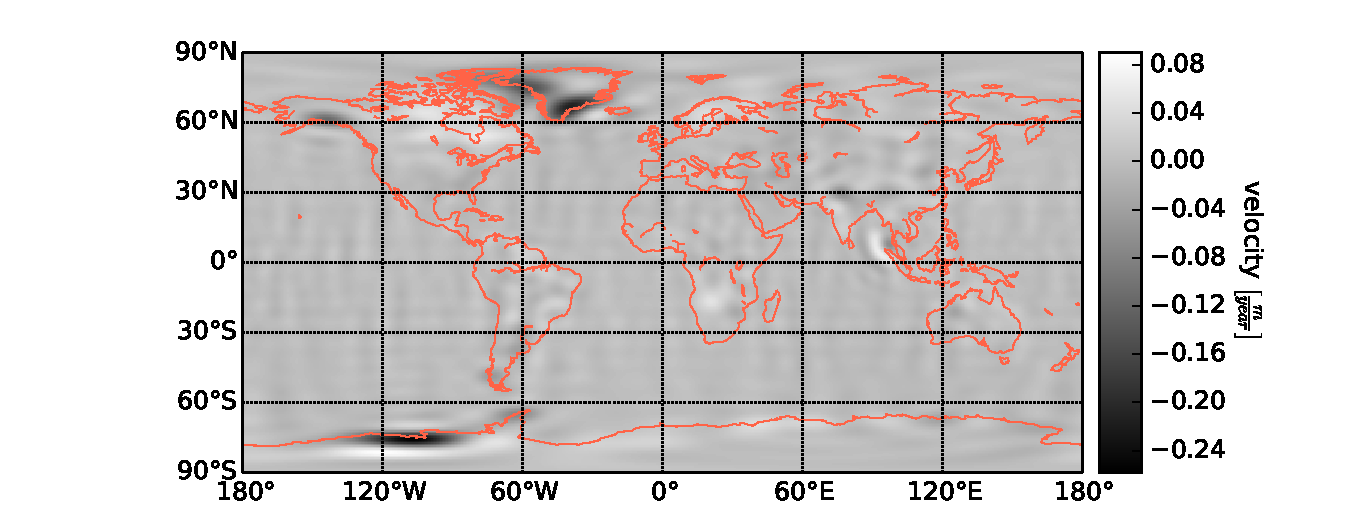
\includegraphics[width=\textwidth]{figures/ols-world-parameter-vel}
	\caption{Estimated velocity ($t$) parameters}
	\label{fig:ols-world-parameter-vel}
\end{figure}

\begin{figure}[H]
	\centering
	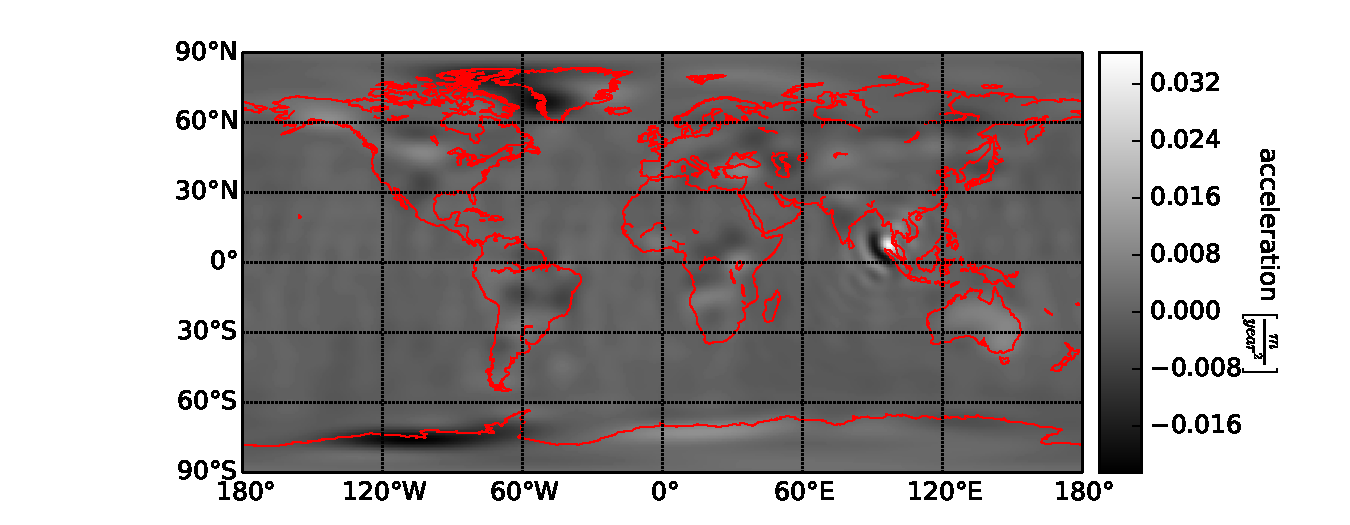
\includegraphics[width=\textwidth]{figures/ols-world-parameter-acc}
	\caption{Estimated acceleration ($\frac{1}{2} t^2$) parameters}
	\label{fig:ols-world-parameter-acc}
\end{figure}

The first two figures (Figure \ref{fig:ols-world-parameter-vel} and Figure \ref{fig:ols-world-parameter-acc}) shows that, generally there is a mass loss at both Greenland and the South Pole and that it is accelerating. However interestingly enough the East Coast of Greenland do not show any acceleration, maybe even a slight deceleration of the mass loss (a positive value).

On both figures there is also a circular pattern at Thailand (10 N, 95 E), which is caused by the infamous earthquake of the 26th December 2004, resulting in significant changes in the mass distribution, thus affecting the data from GRACE.
\begin{figure}[H]
	\centering
	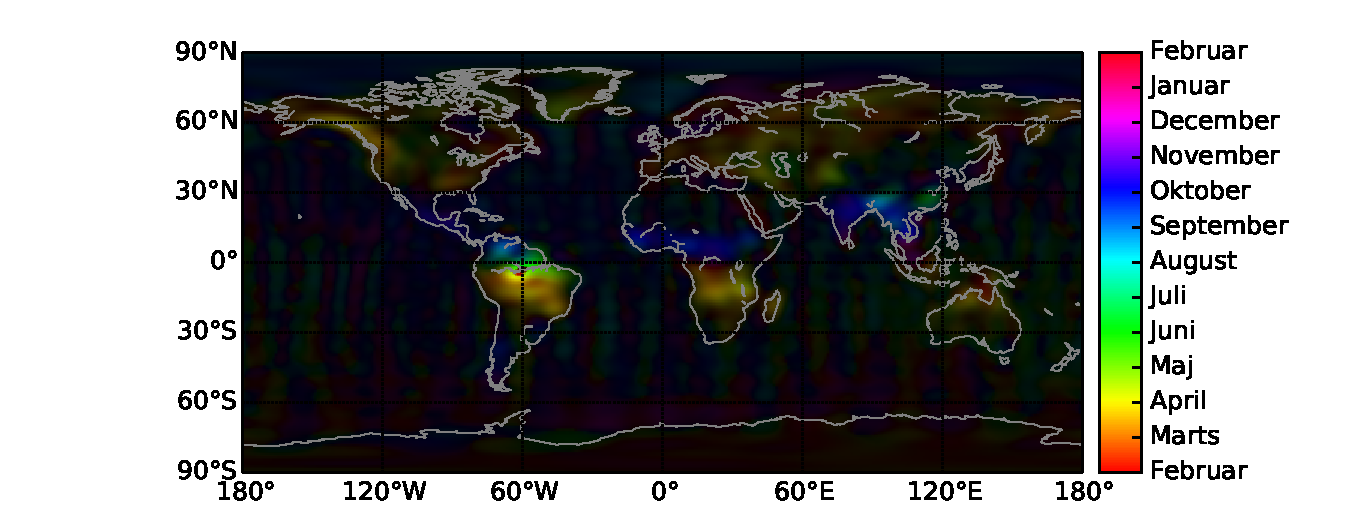
\includegraphics[width=\textwidth]{figures/ols-world-parameter-year}
	\caption{Estimated phase and amplitude for the yearly seasons.}
	\label{fig:ols-world-parameter-year}
\end{figure}

The seasonal trends do not reveal any information about mass loss due to ice melting, since this is something which will continue to have effect for many years. However it does affect the estimation of the velocity and acceleration. Also having more season related terms in the OLS regression than necessary, will result in fewer degrees of freedom.

In Figure \ref{fig:ols-world-parameter-year} it is seen from the intensity, that the South Pole do not have a strong yearly seasonal trend unlike Greenland. It also appears that it is primarily the East Coast of Greenland which has a yearly seasonal trend. The strongest seasonal trend appears in South America, and this is due to the rain season. This rain also takes quite some time to reach the ocean, thus causing the phase gradient.

\paragraph{Performance} 

As a measure of  model performance the root mean squared error has been calculated for each position.
\begin{figure}[H]
	\centering
	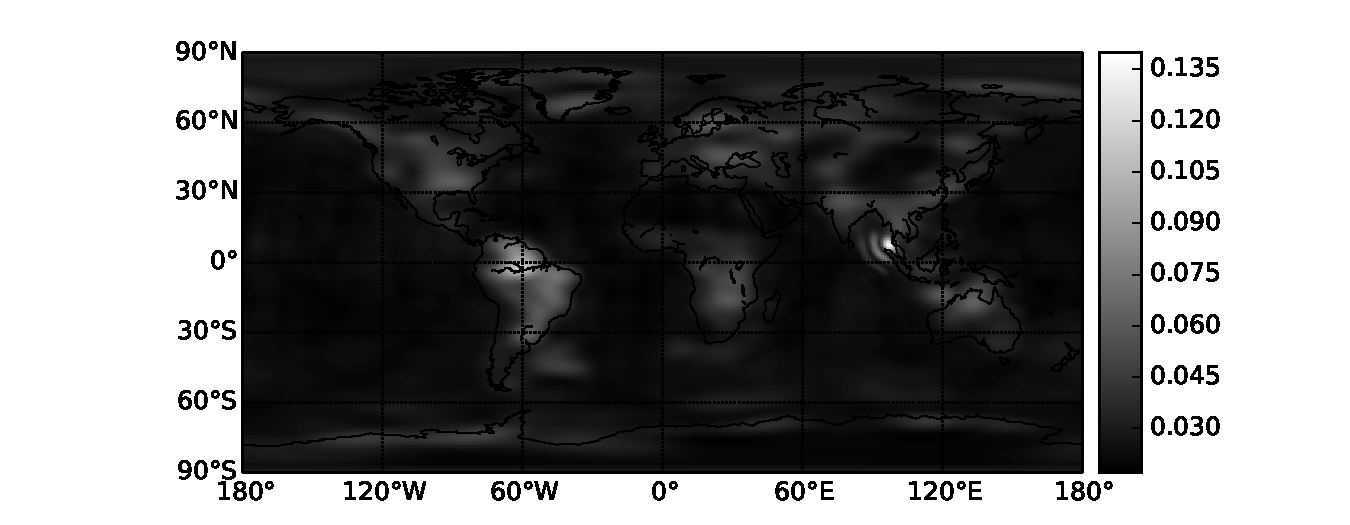
\includegraphics[width=\textwidth]{figures/ols-world-performance-rmse}
	\caption{RMSE for each position.}
	\label{fig:ols-world-performance-rmse}
\end{figure}

From \ref{fig:ols-world-performance-rmse} it is seen that the hardest places to fit are South America and Thailand. In South America it is especially around the Amazon River that the RMSE is high. This suggests that it is caused by the rain seasons, since this is also the place with the highest amplitude of the yearly seasonal term. It's a bit odd that this is so hard to fit, since the model does support seasonal trends. One explanation could be that this OLS model assumes that the season are equally long and with identical phases each year, which is not very likely. The circular pattern around Thailand is no surprise, since the OLS model was never meant to fit this distortion.

Neither of these issues are related to the ice melting, which makes them less important. However the East Coast of Greenland and the South Pole also show a relative higher RMSE, when comparing to the ocean or the nearby land, which is less than ideal. The fact that it is primarily the East Coast of Greenland and not the west coast, suggests that the issues are related to the seasons, just like with South America. This was also something observed, when looking at the specific location's time series.

\paragraph{Standard diagnostics} Recalling that $\mathrm{Var}[\hat{Y}_i] = \sigma^{2} H_{ii}$ and $\mathrm{D}[\hat{\beta}] = \sigma^{2} V \Sigma^{-2} V^T$ the diagonal of $H$ and $V \Sigma^{-2} V^T$ are both important to examine. This will identify any days and parameters with high variance.

\begin{figure}[H]
	\centering
	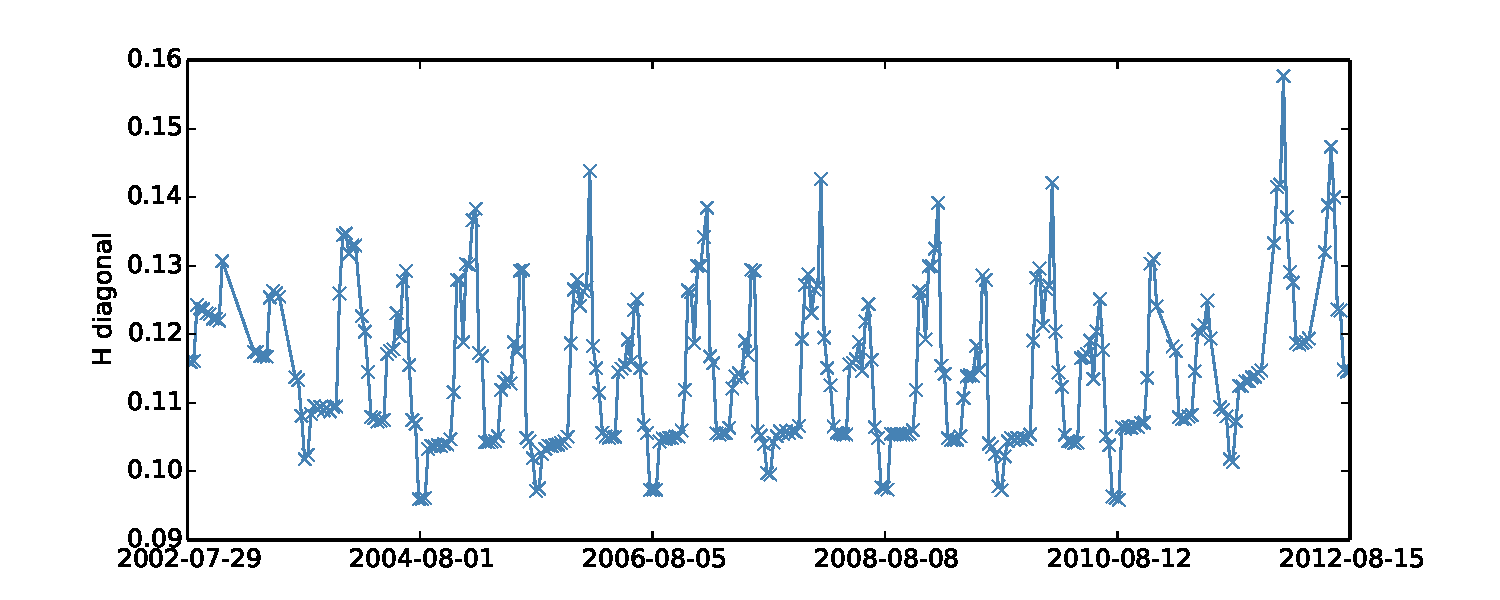
\includegraphics[width=\textwidth]{figures/ols-world-diagnostics-diagH}
	\caption{The diagonal of $H$ will reveal any days with a high variance.}
	\label{fig:ols-world-performance-diagH}
\end{figure}

The variances shown in Figure \ref{fig:ols-world-performance-diagH} are not very big, the highest is $0.16$ and recalling that the 95\% confidence interval can be approximated by $\hat{Y}_i \pm 2 \cdot \hat{\sigma} \sqrt{\mathrm{Var}[\hat{Y}_i]}$. The maximal confidence interval becomes $\hat{Y}_i \pm 2 \cdot 0.135 \cdot \sqrt{0.16} = \hat{Y}_i \pm 0.108$, which is small when comparing to the EWH values, which range from $1$ to $-3$. What is odd about $\mathrm{diag}(H)$ is that there appears be some parts in each year there are more difficult to predict than others. \todo{Why is this}

\begin{figure}[H]
	\centering
	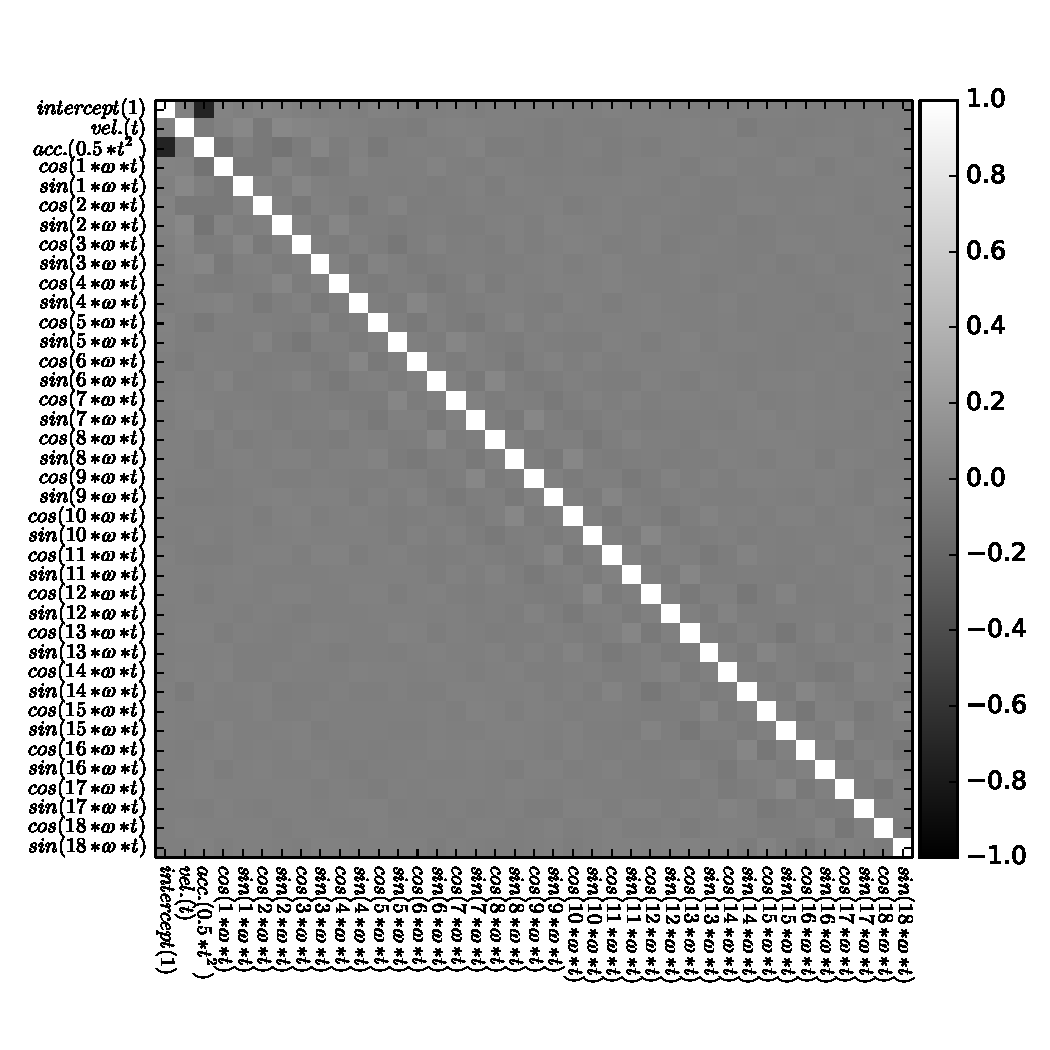
\includegraphics[height=9cm]{figures/ols-world-diagnostics-cov}
	\caption{$V \Sigma^{-2} V^T$ will reveal correlated parameter and parameters with high variance.}
	\label{fig:ols-world-performance-cov}
\end{figure}

From Figure \ref{fig:ols-world-performance-cov} it is seen that the parameters are nicely uncorrelated and while the seasonal parameters have a slightly high variance when comparing to their values, the velocity and acceleration parameters are practically zero.
\begin{table}[H]
\centering
\begin{tabular}{r|c c c}
	name & $\mathrm{Var}[\hat{\beta}_i]$ \\ \hline
	$vel. (t)$ & $2.91390457 \cdot 10^{-09}$  \\
	$acc. (0.5 \cdot t^2)$ & $1.29525397 \cdot 19^{-14}$
\end{tabular}
\caption{Variance of the velocity and acceleration parameters}
\end{table}

\paragraph{p-values} Just as for the selected positions, inspecting the p-values can tell which OLS terms are important.

\begin{figure}[H]
	\centering
	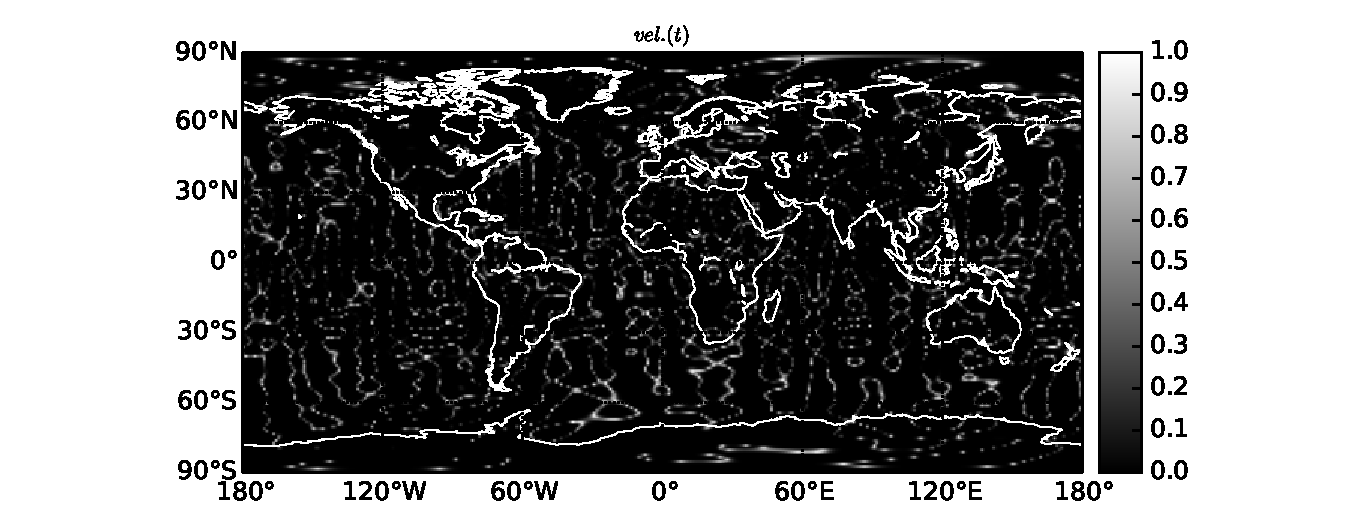
\includegraphics[width=\textwidth]{figures/ols-world-diagnostics-pvalue-1}
	\caption{p-values for the velocity parameter.}
	\label{fig:ols-world-diagnostics-pvalue-1}
\end{figure}

\begin{figure}[H]
	\centering
	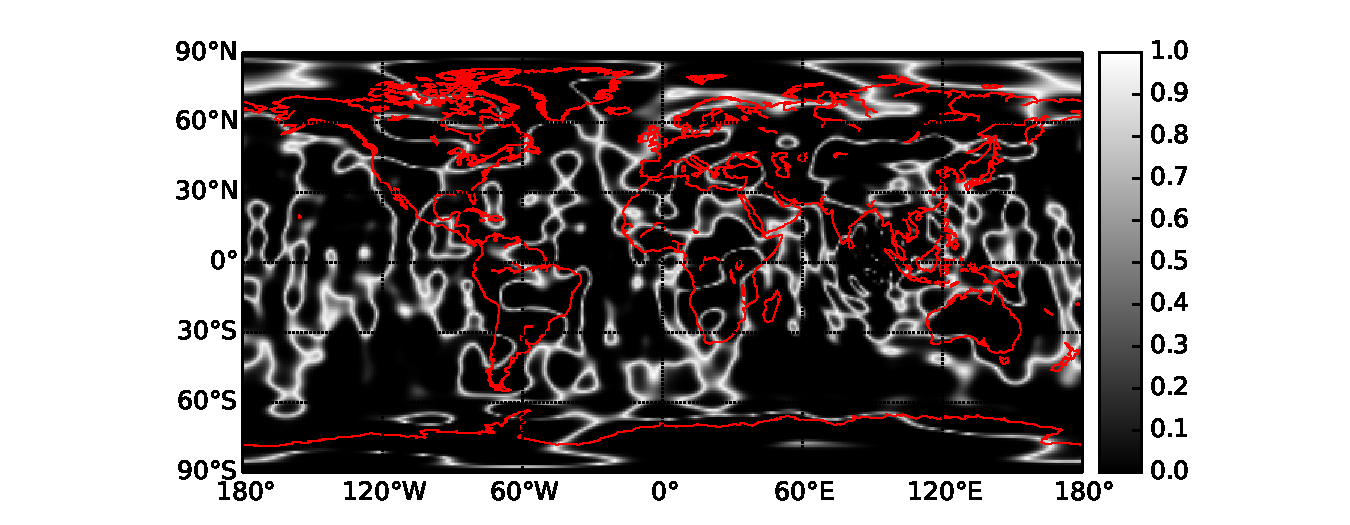
\includegraphics[width=\textwidth]{figures/ols-world-diagnostics-pvalue-2}
	\caption{p-values for the acceleration parameter.}
	\label{fig:ols-world-diagnostics-pvalue-2}
\end{figure}

There is not much surprise in either Figure \ref{fig:ols-world-diagnostics-pvalue-1} or Figure \ref{fig:ols-world-diagnostics-pvalue-2}. Both the velocity and the acceleration appears to be significant pretty much everywhere. The places where it is not, is where there is a sign shift thus causing the p-value gradient. This is particularly apparent with the acceleration. One odd detail is that also on the ocean, the velocity and acceleration parameters appears to be significantly different from zero. In the ocean there is no reason to expect a steady mass change, though when looking at actual values it's seen that there is a slight slope. This quite small slope then becomes significant, due to the very small variance of the velocity and acceleration parameters. 

\begin{figure}[H]
	\centering
	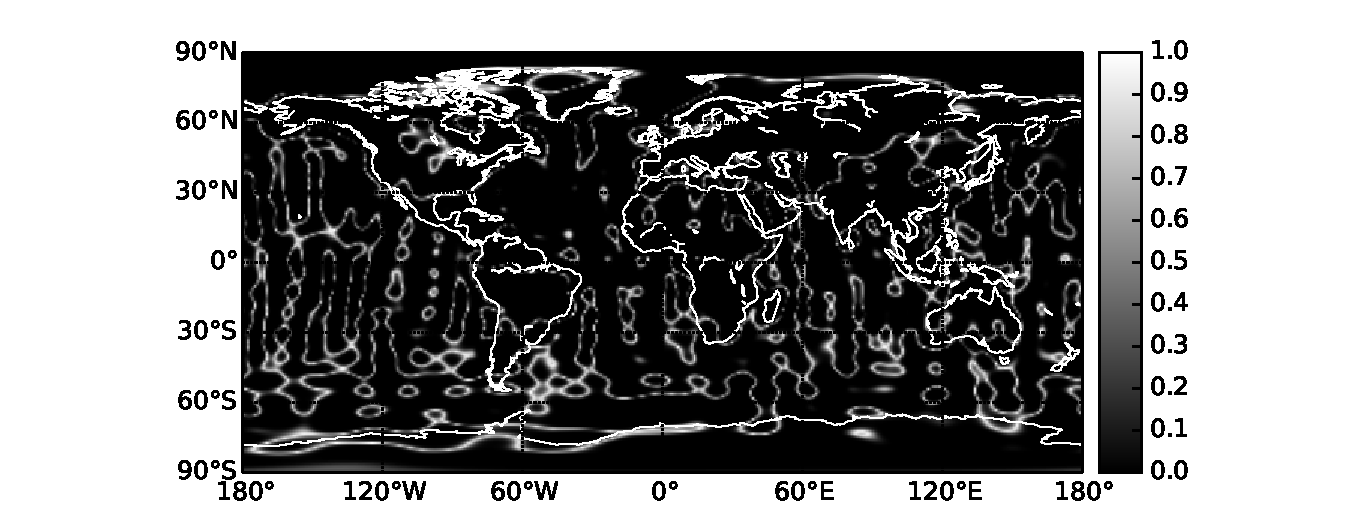
\includegraphics[width=\textwidth]{figures/ols-world-diagnostics-pvalue-3}
	\caption{p-values for the yearly seasonal cosine parameter.}
	\label{fig:ols-world-diagnostics-pvalue-3}
\end{figure}

\begin{figure}[H]
	\centering
	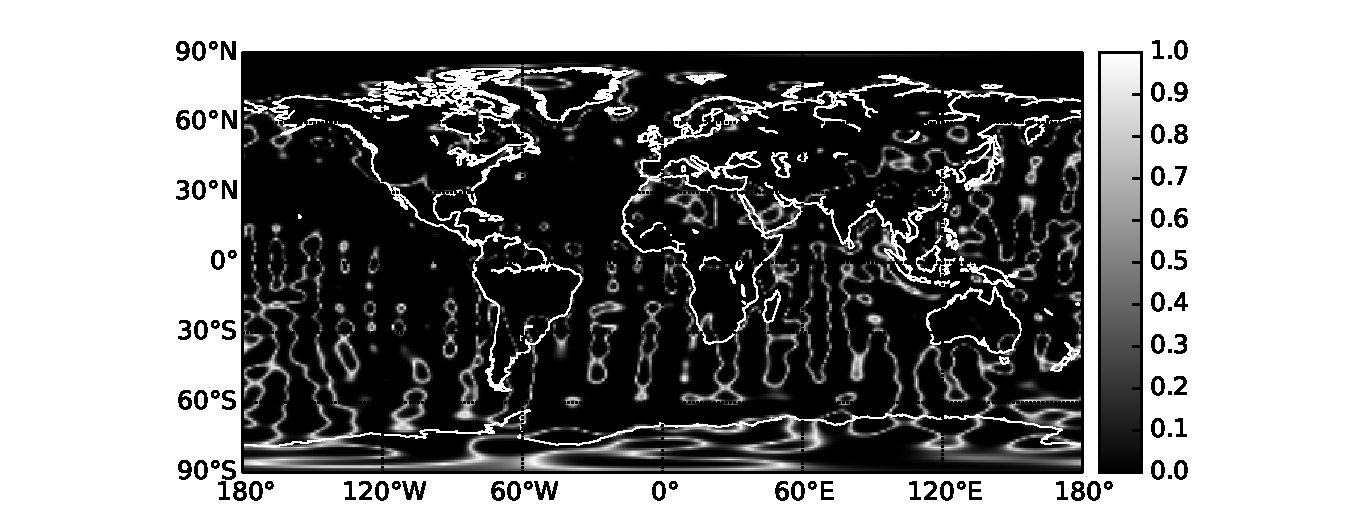
\includegraphics[width=\textwidth]{figures/ols-world-diagnostics-pvalue-4}
	\caption{p-values for the yearly seasonal sine parameter.}
	\label{fig:ols-world-diagnostics-pvalue-4}
\end{figure}

Also the yearly seasonal parameters are significant pretty much everywhere. For these parameters it makes more sense that they are significant in the ocean.

\todo{How many parameters should be analysed}

\paragraph{PCA of residuals}

By computing the principal component for the OLS residuals, it is some times possible to discover patterns in the residuals. As with all PCA one the first couple of principal components are valuable to look at.
\begin{figure}[H]
\centering
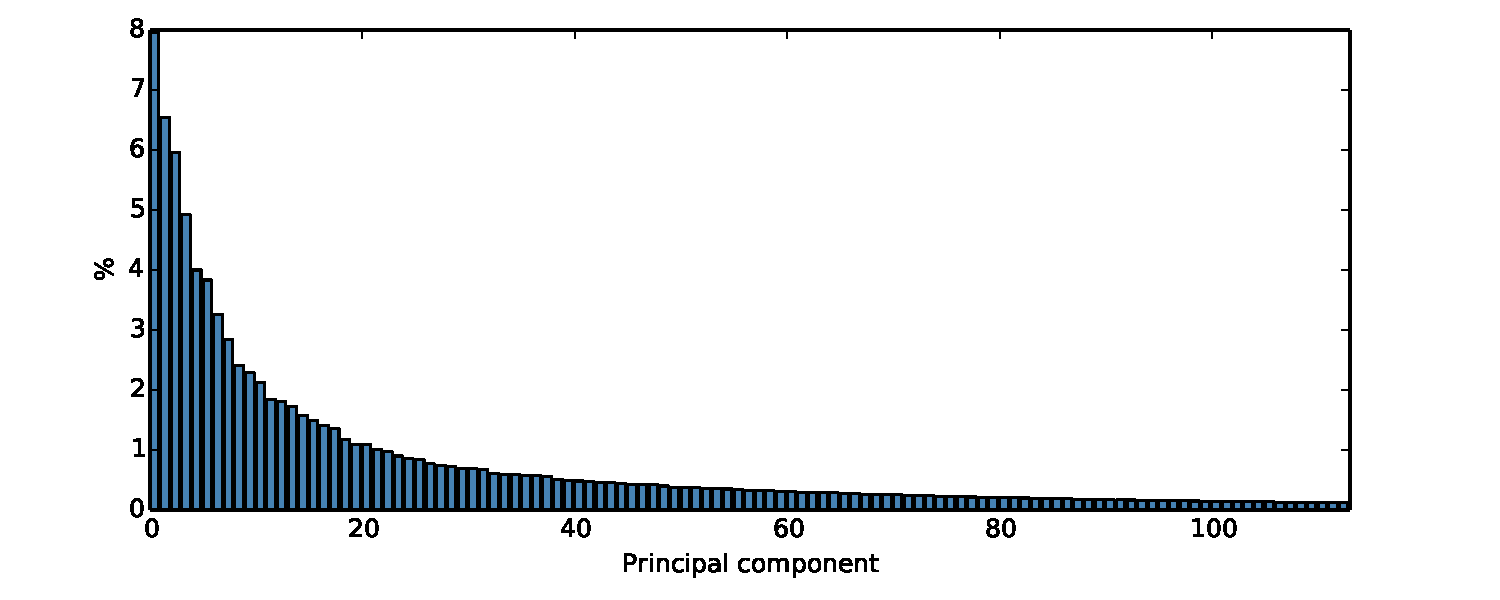
\includegraphics[width=1.0\textwidth]{figures/ols-pca-explained}
\caption{Variance explained by each principal component}
\label{fig:ols-pca-explained}
\end{figure}

If the PCA had been used on the original GRACE data, first couple of PCs would likely have explained most of the variance. However since this PCA is done on the residuals, the primary data is hopefully noise, thus no particularly direction shows a lot of variance. The shape of Figure \ref{fig:ols-pca-explained} indicates that there is a lot of noise, but that there also exists residuals there isn't just noise.

Plotting the first principal component score and loading, one gets:
\begin{figure}[H]
\centering
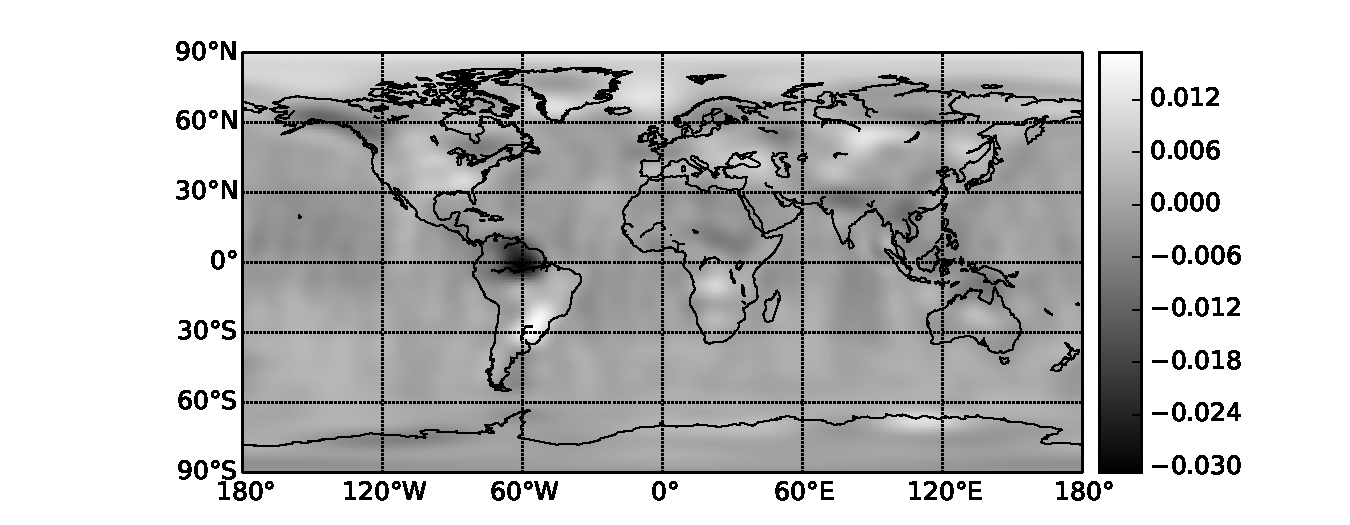
\includegraphics[width=1.0\textwidth]{figures/ols-pca-score-0}
\caption{PC score for the first principal component}
\label{fig:ols-pca-score-0}
\end{figure}

From Figure \ref{fig:ols-pca-score-0} its seen that there is some residuals at South America there is unlikely to be caused by noise. This could be because of the rainy seasons, since those are poorly modeled using this OLS regression. If that is the case one should expect Figure \ref{fig:ols-pca-loading-0} to show some yearly periodic trend. Unfortunately this do not seam to be the case. \todo{Now what?}

\begin{figure}[H]
\centering
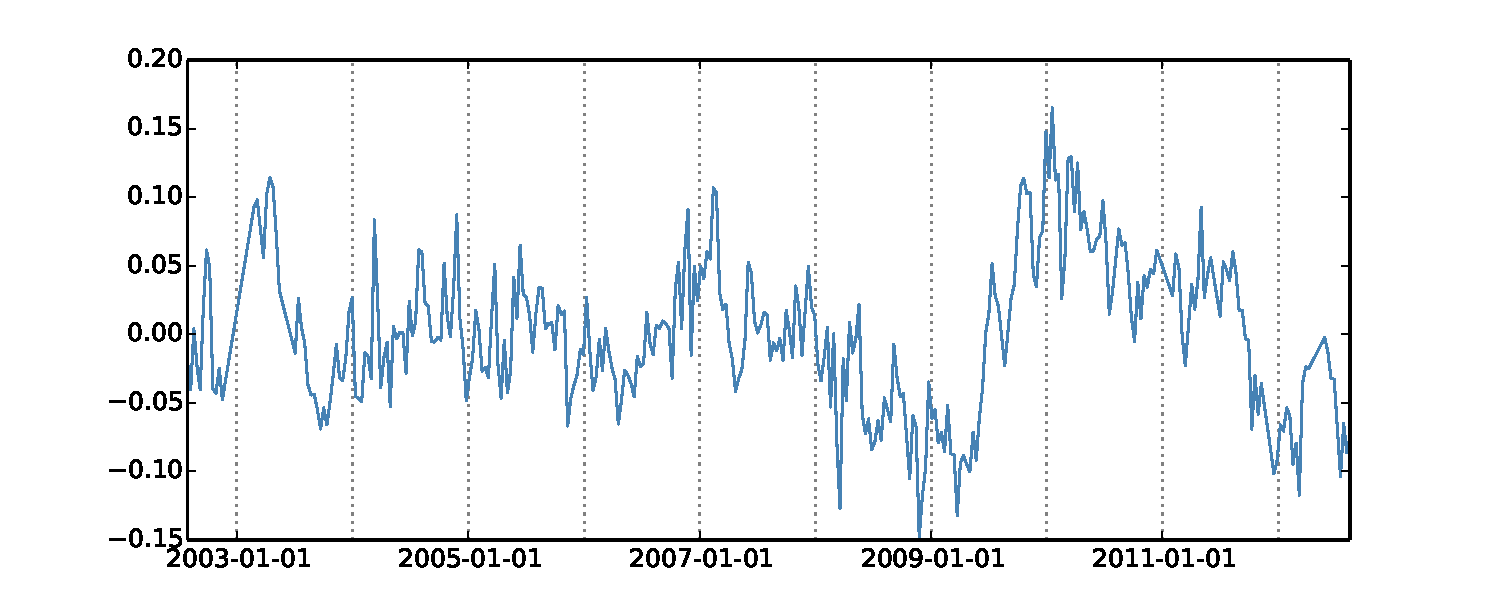
\includegraphics[width=1.0\textwidth]{figures/ols-pca-loading-0}
\caption{PC loading for the first principal component}
\label{fig:ols-pca-loading-0}
\end{figure}

Plotting the second principal component score and loading, one gets:
\begin{figure}[H]
\centering
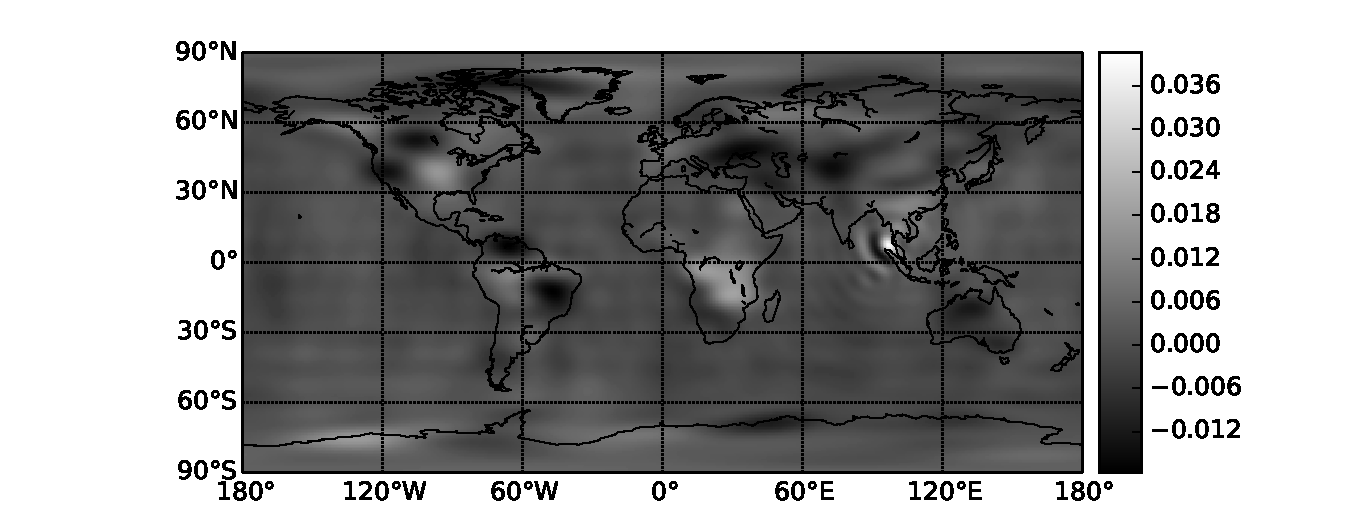
\includegraphics[width=1.0\textwidth]{figures/ols-pca-score-1}
\caption{PC score for the second principal component}
\label{fig:ols-pca-score-1}
\end{figure}

\begin{figure}[H]
\centering
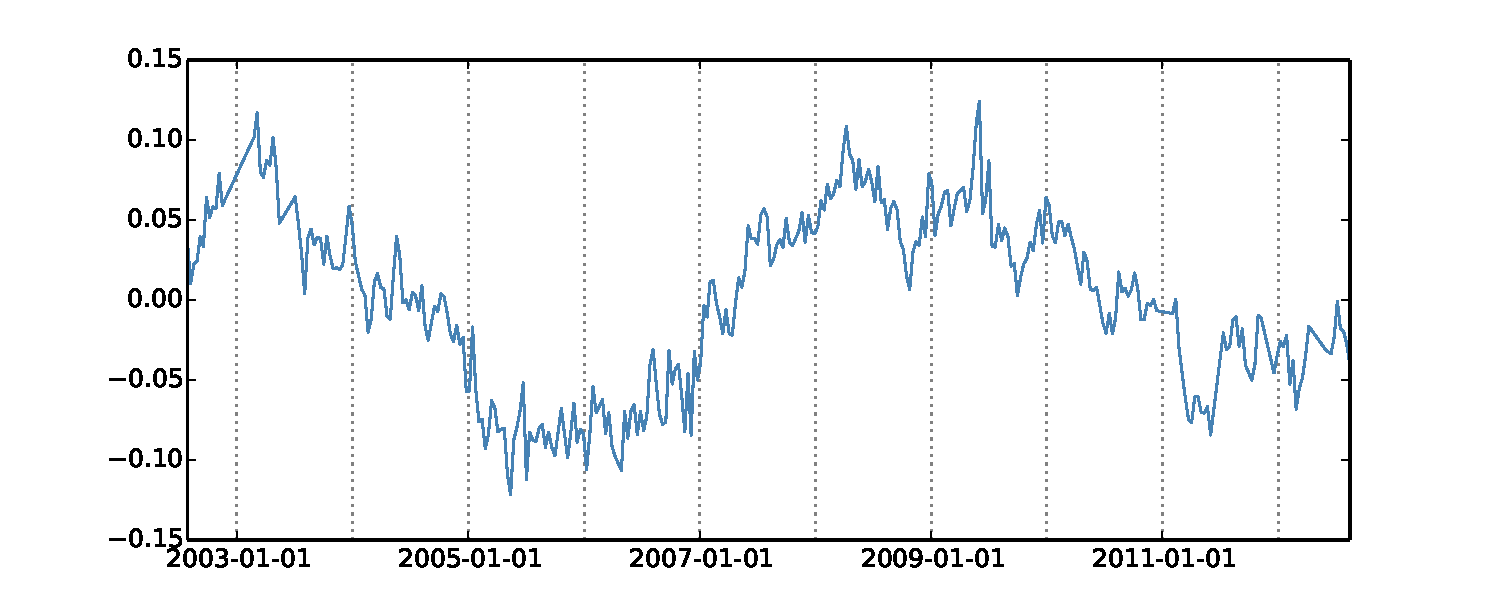
\includegraphics[width=1.0\textwidth]{figures/ols-pca-loading-1}
\caption{PC loading for the second principal component}
\label{fig:ols-pca-loading-1}
\end{figure}

In Figure \ref{fig:ols-pca-score-1} a strong circular pattern appears. This is the caused by the earthquake near Thailand in 2004 and can't be modeled by this OLS regression, so those residuals are expected. A bit strange is that \ref{fig:ols-pca-loading-1} indicates that the residuals not only comes from 2002 to 2004 but also around 2006 and 2009.

More important do Figure \ref{fig:ols-pca-score-1} also show some residuals near west Greenland, this is not ideal since this is one of the areas this report attempts to analyze.
